\documentclass[aspectratio=169,11pt]{ctexbeamer}

\usetheme{Warsaw}
\setbeamertemplate{navigation symbols}{}
\setbeamertemplate{headline}{}

\usepackage{amsmath}
\usepackage{amssymb}
\usepackage{booktabs}
\usepackage{tabularx}
\usepackage{fancyvrb}
\usepackage{xcolor}
\usepackage{graphicx}
\usepackage{tikz}
\usetikzlibrary{arrows.meta,positioning}

\definecolor{codebg}{RGB}{248,248,248}
\definecolor{deepblue}{RGB}{37,99,235}
\definecolor{darkgreen}{RGB}{22,101,52}
\definecolor{warmorange}{RGB}{217,119,6}
\setbeamercolor{block body}{bg=codebg,fg=black}
\setbeamercolor{block title}{bg=deepblue,fg=white}

\title{三维数据可视化}
\author{crazyfish}
\date{\today}

\newcommand{\R}{\mathbb R}
\newcommand{\vx}{\mathbf x}
\newcommand{\vv}{\mathbf v}
\newcommand{\dd}{\mathrm d}

\begin{document}

\begin{frame}
  \titlepage
\end{frame}

\begin{frame}{合集结构}
  本合集合并五个项目的完整 slide，每个项目作为独立的 Part：

  \begin{enumerate}
    \item \textbf{Part I.} \texttt{basic\_3d} — 三维绘图、坐标系、相机与光照
    \item \textbf{Part II.} \texttt{colorad} — Colorado 数字高程模型 + 影像贴图
    \item \textbf{Part III.} \texttt{water\_molecule} — 电子密度等值面
    \item \textbf{Part IV.} \texttt{weather\_simulation} — 云水标量场 + 风速矢量场 + 流速线
    \item \textbf{Part V.} \texttt{medical\_mri} — 头部 MRI 体数据 + 窗位窗宽 + 切片
  \end{enumerate}

  \begin{block}{共同主线}
    五个项目均基于 OpenDX 格式 + Plotly/Dash 技术栈。
    从解析几何 $\to$ 表面 $\to$ 标量场 $\to$ 矢量场 $\to$ 体数据，复杂度递增，底层管线一致。
  \end{block}
\end{frame}

\begin{frame}[fragile]{Dash：本合集统一的交互框架}
  \small
  \texttt{Dash} 是 Plotly 推出的 Python Web 应用框架。五个项目均用 Dash 把 Plotly 图表包装成可在浏览器中实时交互探索的应用，无需手写 HTML/JS。

  \begin{columns}
    \begin{column}{0.48\linewidth}
      \begin{block}{技术栈分层}
        \begin{itemize}
          \item 前端：React + Plotly.js
          \item 后端：Flask (WSGI)
          \item Python 端：声明式组件 + 回调
          \item 通过浏览器访问（默认 \texttt{http://127.0.0.1:8050}）
        \end{itemize}
      \end{block}
    \end{column}
    \begin{column}{0.48\linewidth}
      \begin{block}{核心组件}
        \begin{itemize}
          \item \texttt{html.Div}：页面布局容器
          \item \texttt{dcc.Slider / Checklist}：输入控件
          \item \texttt{dcc.Graph}：嵌入 Plotly 图表
          \item \texttt{@app.callback}：响应函数
          \item \texttt{uirevision}：跨更新保留视角
        \end{itemize}
      \end{block}
    \end{column}
  \end{columns}

  \begin{block}{统一代码骨架}
\begin{Verbatim}[fontsize=\scriptsize]
app = Dash(__name__)
app.layout = html.Div([dcc.Slider(id="s", ...), dcc.Graph(id="g")])
@app.callback(Output("g", "figure"), Input("s", "value"))
def update(v): return build_plotly_figure(v)
app.run(host="127.0.0.1", port=8050)
\end{Verbatim}
  \end{block}
\end{frame}

\part{basic\_3d: 三维绘图与可视化基本概念}

\begin{frame}{本讲目标}
  通过一个最小三维场景理解三维绘图的核心组成。

  \begin{itemize}
    \item 物体：单位立方体与单位球。
    \item 空间：坐标轴、尺度、中心与方向。
    \item 观察：相机位置、视角与投影。
    \item 渲染：颜色、光源、漫反射、镜面反射与粗糙度。
    \item 交互：滑杆、鼠标旋转、实时更新。
  \end{itemize}
\end{frame}

\begin{frame}[fragile]{运行示例}
  本讲围绕当前目录中的 Dash + Plotly 示例展开。

  \begin{block}{启动命令}
\begin{Verbatim}[fontsize=\small]
conda activate ai4math-vis
python basic_3d/plotly_unit_cube_demo.py
\end{Verbatim}
  \end{block}

  \begin{block}{浏览器地址}
\begin{Verbatim}[fontsize=\small]
http://127.0.0.1:8051
\end{Verbatim}
  \end{block}

  \begin{itemize}
    \item \texttt{Object} 可切换单位立方体与单位球。
    \item \texttt{Lighting} 控制光源位置与材质响应。
    \item 鼠标拖动三维图会同步更新相机位置滑杆。
  \end{itemize}
\end{frame}

\section{三维数据}

\begin{frame}{三维绘图首先是空间数据}
  三维图不是“二维图变立体”，而是数据中真的包含空间结构。

  \begin{table}
    \centering
    \begin{tabularx}{0.9\linewidth}{lllX}
      \toprule
      对象 & 数据 & Plotly 图元 & 典型用途 \\
      \midrule
      点 & \((x,y,z)\) & \texttt{Scatter3d} & 采样点、粒子、传感器 \\
      线 & 点序列 & \texttt{Scatter3d} & 轨迹、边框、流线 \\
      面 & 网格或三角片 & \texttt{Surface/Mesh3d} & 几何边界、地形、等值面 \\
      体 & 三维数组 & \texttt{Volume/Isosurface} & 医学、流体、标量场 \\
      \bottomrule
    \end{tabularx}
  \end{table}
\end{frame}

\begin{frame}{坐标系：三维可视化的参照物}
  三维对象需要放在明确的坐标系中。

  \begin{itemize}
    \item 坐标轴给出方向：\(x\)、\(y\)、\(z\)。
    \item 刻度给出尺度：一个单位到底有多大。
    \item 中心位置决定光源、相机和旋转的参照。
    \item 当前示例中：
      \begin{itemize}
        \item 单位立方体：\([0,1]\times[0,1]\times[0,1]\)。
        \item 单位球：球心 \((0,0,0)\)，半径 \(1\)。
      \end{itemize}
  \end{itemize}
\end{frame}

\begin{frame}{单位立方体：最小的三维几何模型}
  单位立方体适合解释三维几何的基本元素。

  \begin{columns}
    \begin{column}{0.48\linewidth}
      \begin{itemize}
        \item 8 个顶点。
        \item 12 条边。
        \item 6 个面。
        \item 每个面有固定法向。
      \end{itemize}
    \end{column}
    \begin{column}{0.48\linewidth}
      \begin{block}{六个面的法向}
        \[
        \pm\mathbf e_x,\quad
        \pm\mathbf e_y,\quad
        \pm\mathbf e_z
        \]
      \end{block}
      面法向是判断“面是否朝向光源”的关键。
    \end{column}
  \end{columns}
\end{frame}

\begin{frame}{单位球：连续曲面的代表}
  单位球适合解释曲面、法向连续变化和高光。

  \begin{block}{单位球方程}
    \[
    x^2+y^2+z^2=1
    \]
  \end{block}

  \begin{itemize}
    \item 球面上每一点都有自己的法向。
    \item 对单位球，点 \(\mathbf p=(x,y,z)\) 的法向就是 \(\mathbf n=\mathbf p\)。
    \item 因为法向连续变化，漫反射和镜面反射在球面上更容易观察。
  \end{itemize}
\end{frame}

\section{绘制管线}

\begin{frame}{三维绘图管线}
  从数学对象到屏幕图像，一般经历如下步骤。

  \begin{center}
    \begin{tikzpicture}[
      node distance=0.75cm,
      box/.style={draw, rounded corners=2pt, align=center, minimum width=1.75cm, minimum height=0.72cm},
      arr/.style={-{Stealth[length=2.2mm]}, thick}
    ]
      \node[box] (data) {数据\\坐标/网格};
      \node[box, right=of data] (geom) {几何\\点/线/面};
      \node[box, right=of geom] (view) {相机\\视角/投影};
      \node[box, right=of view] (shade) {光照\\颜色/材质};
      \node[box, right=of shade] (screen) {屏幕\\交互显示};
      \draw[arr] (data) -- (geom);
      \draw[arr] (geom) -- (view);
      \draw[arr] (view) -- (shade);
      \draw[arr] (shade) -- (screen);
    \end{tikzpicture}
  \end{center}

  \begin{itemize}
    \item Plotly 负责把图元渲染到浏览器中的 WebGL 画布。
    \item Dash 负责把滑杆、下拉框等控件连接到 Python 回调。
  \end{itemize}
\end{frame}

\begin{frame}[fragile]{Plotly 图元：\texttt{Surface} 与 \texttt{Scatter3d}}
  \footnotesize
  当前示例主要使用两个三维图元。

  \begin{block}{球面或细分面}
\begin{Verbatim}[fontsize=\scriptsize]
go.Surface(
    x=x_values,
    y=y_values,
    z=z_values,
    surfacecolor=intensities,
)
\end{Verbatim}
  \end{block}

  \begin{block}{光源点与虚线}
\begin{Verbatim}[fontsize=\scriptsize]
go.Scatter3d(
    x=[light_x, target_x],
    y=[light_y, target_y],
    z=[light_z, target_z],
    mode="markers+lines+text",
)
\end{Verbatim}
  \end{block}
\end{frame}

%% \begin{frame}{为什么不用 Plotly 内部 \texttt{lightposition}}
%%   本例采用显式光照计算，而不是完全依赖 Plotly 内部光照。

%%   \begin{itemize}
%%     \item Plotly 的三维光照会经过内部矩阵变换。
%%     \item 可见的“光源点”和内部 shader 光源方向不一定直观一致。
%%     \item 教学时更需要“光源在哪边，哪边更亮”的稳定对应关系。
%%     \item 因此本例直接计算每个面或每个采样点的亮度，再把亮度映射为颜色。
%%   \end{itemize}
%% \end{frame}

\section{相机}

\begin{frame}{相机：决定我们从哪里看}
  三维场景最终仍显示在二维屏幕上，相机定义观察方式。

  \begin{itemize}
    \item \texttt{camera.eye}：相机所在位置。
    \item \texttt{camera.center}：观察中心偏移。
    \item \texttt{camera.up}：画面中“上方”的方向。
    \item 鼠标旋转三维图，本质上是在改变相机视角。
  \end{itemize}

  \begin{block}{当前示例}
    鼠标调整相机后，\texttt{Camera X/Y/Z} 滑杆会同步更新。
  \end{block}
\end{frame}

\begin{frame}[fragile]{相机参数示意}
  Plotly 中的三维相机通常写在 \texttt{layout.scene.camera} 中。

  \begin{block}{示例结构}
\begin{Verbatim}[fontsize=\small]
scene={
    "camera": {
        "eye": {"x": camera_x, "y": camera_y, "z": camera_z},
        "center": {"x": 0, "y": 0, "z": 0},
    }
}
\end{Verbatim}
  \end{block}

  \begin{itemize}
    \item 相机离物体越远，物体看起来越小。
    \item 相机绕物体移动，看到的亮面和高光也会变化。
  \end{itemize}
\end{frame}

\section{光照与材质}

\begin{frame}{光照模型的基本思想}
  当前示例使用简化的局部光照模型。

  \begin{block}{核心公式}
    \[
    I =
    A
    + D\max(\mathbf n\cdot \mathbf l,0)
    + S\,H
    + F\,E
    \]
  \end{block}

  \begin{itemize}
    \item \(\mathbf n\)：表面法向。
    \item \(\mathbf l\)：从表面指向光源的单位方向。
    \item \(H\)：镜面高光项。
    \item \(E\)：边缘视角反光项。
  \end{itemize}
\end{frame}

\begin{frame}{Ambient：环境光}
  \texttt{Ambient 环境光} 不是光源强度，而是基础亮度。

  \begin{itemize}
    \item 不依赖光源方向。
    \item 所有面都会获得一部分亮度。
    \item 值越大，阴影越浅，对比越弱。
    \item 值越小，背光面越暗，光照方向更明显。
  \end{itemize}

  \begin{block}{教学观察}
    把 \texttt{Ambient} 降低，再移动光源，光照方向最明显。
  \end{block}
\end{frame}

\begin{frame}{Diffuse：漫反射}
  \texttt{Diffuse 漫反射} 是最直观的受光效果。

  \begin{block}{Lambert 漫反射}
    \[
    I_D = D\max(\mathbf n\cdot \mathbf l,0)
    \]
  \end{block}

  \begin{itemize}
    \item 面朝向光源：\(\mathbf n\cdot\mathbf l\) 大，亮。
    \item 面背向光源：\(\mathbf n\cdot\mathbf l<0\)，不接受漫反射。
    \item 单位立方体中，移动光源可以直接观察哪个面变亮。
  \end{itemize}
\end{frame}

\begin{frame}{Specular 与 Roughness：高光和粗糙度}
  \texttt{Specular 镜面反射} 控制高光强度，\texttt{Roughness 粗糙度} 控制高光范围。

  \begin{itemize}
    \item \texttt{Specular} 越大，高光越亮。
    \item \texttt{Roughness} 越小，高光越集中。
    \item \texttt{Roughness} 越大，高光越宽、越钝。
    \item 球面比立方体更适合观察连续高光。
  \end{itemize}

  \begin{block}{课堂操作}
    切换到单位球，把 \texttt{Specular} 从 0 拉到 2，再调节 \texttt{Roughness}。
  \end{block}
\end{frame}

\begin{frame}{Fresnel：斜视角反光}
  \texttt{Fresnel 菲涅尔} 描述反射强度随观察角度变化。

  \begin{itemize}
    \item 正对表面时，边缘反光较弱。
    \item 接近掠射角观察时，边缘反光更强。
    \item 在球面边缘区域更容易观察。
    \item 本例中的 Fresnel 是近似，不是完整物理渲染。
  \end{itemize}
\end{frame}

\section{交互}

\begin{frame}{为什么要交互}
  三维概念很难只靠静态图说明。

  \begin{itemize}
    \item 旋转相机：理解三维结构。
    \item 移动光源：理解法向和受光方向。
    \item 调材质参数：理解渲染风格。
    \item 切换对象：比较平面几何与曲面几何。
  \end{itemize}

  \begin{block}{本例的关键交互}
    所有滑杆使用拖动时更新，参数变化可以连续观察。
  \end{block}
\end{frame}

%% \begin{frame}[fragile]{Dash 回调：控件驱动图像更新}
%%   Dash 的核心思想是：输入控件变化，回调函数重新生成图形。

%%   \begin{block}{概念结构}
%% \begin{Verbatim}[fontsize=\small]
%% @app.callback(
%%     Output("cube-graph", "figure"),
%%     Input("object-shape", "value"),
%%     Input("light-x", "value"),
%%     Input("ambient", "value"),
%%     ...
%% )
%% def update_cube(...):
%%     controls = normalize_controls(...)
%%     return make_figure_from_controls(controls)
%% \end{Verbatim}
%%   \end{block}
%% \end{frame}

\begin{frame}{演示顺序建议}
  \begin{enumerate}
    \item 先只看单位立方体，打开坐标轴，关闭边框。
    \item 移动光源，观察哪一个面变亮。
    \item 降低 \texttt{Ambient}，增强明暗对比。
    \item 切换到单位球，观察连续明暗变化。
    \item 调节 \texttt{Specular} 和 \texttt{Roughness}，观察高光。
    \item 鼠标旋转相机，观察相机位置对高光的影响。
  \end{enumerate}
\end{frame}

\begin{frame}{从这个例子推广到模拟结果可视化}
  计算模拟结果通常只是把“几何对象”换成更复杂的数据。

  \begin{itemize}
    \item 地形：二维高度场 \(\rightarrow\) 曲面。
    \item 流体：速度向量 \(\rightarrow\) 箭头、流线。
    \item 标量场：温度/密度 \(\rightarrow\) 切片、等值面、体渲染。
    \item 医学图像：三维体素 \(\rightarrow\) 切片与体渲染。
  \end{itemize}

  \begin{block}{不变的核心概念}
    坐标、网格、相机、颜色映射、光照、交互。
  \end{block}
\end{frame}

\begin{frame}{小结}
  三维绘图的基本概念可以用一个很小的场景讲清楚。

  \begin{itemize}
    \item 几何决定物体形状。
    \item 坐标轴决定空间参照。
    \item 相机决定观察方式。
    \item 光源和材质决定明暗与高光。
    \item 交互让参数和视觉结果建立直接联系。
  \end{itemize}

  \begin{block}{本讲示例文件}
    \texttt{basic\_3d/plotly\_unit\_cube\_demo.py}
  \end{block}
\end{frame}

\part{colorad: Colorado 地形数据集}

\begin{frame}{本讲目标}
  了解 Colorado 地形数据集的来源、格式和三维渲染中的关键考量。

  \begin{itemize}
    \item 数据集内容：高程数据 + 航拍影像。
    \item 背景：OpenDX 科学可视化平台的历史。
    \item 格式：二进制数据布局与元数据解析。
    \item 渲染：地形可视化中的高度缩放、光照与性能。
  \end{itemize}
\end{frame}

\section{数据集概述}

\begin{frame}{数据集内容}
  Colorado 地形是 OpenDX 教学样本之一，包含同一地理区域的两个数据层。

  \begin{table}
    \centering
    \begin{tabularx}{0.9\linewidth}{lllX}
      \toprule
      文件 & 大小 & 格式 & 内容 \\
      \midrule
      \texttt{colo\_elev.general} & 109 B & 文本 & 元数据头文件 \\
      \texttt{colorado\_elev.vit} & 157 KB & 二进制 & $400\times400$ 高程 (uint8) \\
      \texttt{colorado.tiff} & 470 KB & TIFF & $400\times400$ RGB 航拍照片 \\
      \bottomrule
    \end{tabularx}
  \end{table}

  \begin{itemize}
    \item 两个数据共享同一个 $400\times400$ 网格。
    \item 高程值范围 $[5, 255]$，均值约 84，标准差约 47。
    \item 航拍照片已经包含自然光照信息。
  \end{itemize}
\end{frame}

\begin{frame}{\texttt{colorado.tiff}：航拍照片实际样貌}
  \centering
  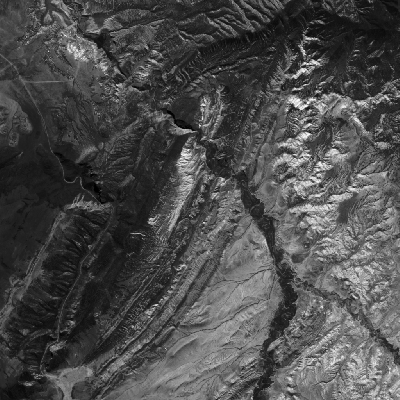
\includegraphics[height=0.72\textheight,keepaspectratio]{colorad/colorado.png}

  \vspace{0.3em}
  \footnotesize
  $400\times 400$ 像素，8-bit sRGB；自然光照与地形纹理已经融合进 RGB 值。
\end{frame}

\begin{frame}{数据背景：OpenDX}
  这个数据集最初来自 IBM 的 Open Visualization Data Explorer (OpenDX)。

  \begin{itemize}
    \item \textbf{起源}：IBM 在 1990 年代开发了 Visualization Data Explorer (DX)，1999 年开源为 OpenDX。
    \item \textbf{定位}：面向科学计算的可视化编程平台，通过连接模块（节点）构建可视化管线。
    \item \textbf{样本数据}：OpenDX 随附多个教学样例，Colorado 地形是其中的地形可视化示例。
    \item \textbf{时间}：该样本来自 1997 年，使用 DX Beta 3.1.4 创建。
  \end{itemize}

  \begin{block}{当前用途}
    在我们的课程中，Colorado 数据被转换为 PyVista/VTK 格式或直接由 Python 读取，
    用于地形渲染教学，无需安装 OpenDX。
  \end{block}
\end{frame}

\begin{frame}{OpenDX 可视化管线（原始示例）}
  原始的 \texttt{Topo.net} 文件描述了如何组合数据与可视化操作。

  \begin{center}
    \begin{tikzpicture}[
      node distance=0.55cm,
      box/.style={draw, rounded corners=2pt, align=center, minimum width=1.3cm, minimum height=0.6cm, font=\footnotesize},
      arr/.style={-{Stealth[length=1.8mm]}, thick}
    ]
      \node[box] (img) {ReadImage\\\scriptsize colorado.tiff};
      \node[box, right=of img] (import1) {Import};
      \node[box, right=of import1] (orient) {Reorient\\对齐网格};
      \node[box, right=of orient] (replace) {Replace\\替换颜色};
      \node[box, right=of replace] (rubber) {RubberSheet\\高度偏移};
      \node[box, right=of rubber] (display) {Display\\地形+影像};

      \node[box, below=of import1] (elev) {Import\\高程数据};
      \draw[arr] (elev) -- (orient);

      \draw[arr] (img) -- (import1);
      \draw[arr] (import1) -- (orient);
      \draw[arr] (orient) -- (replace);
      \draw[arr] (replace) -- (rubber);
      \draw[arr] (rubber) -- (display);
    \end{tikzpicture}
  \end{center}

  \begin{itemize}
    \item \texttt{Reorient}：对齐影像与高程的网格方向。
    \item \texttt{Replace}：将高程值注入影像数据的颜色通道。
    \item \texttt{RubberSheet}：用高程值将二维表面抬升为三维地形。
  \end{itemize}
\end{frame}

\section{数据格式}

\begin{frame}[fragile]{\texttt{.general} 头文件}
  这是整个数据集的入口文件，描述高程文件的存储参数。

  \begin{columns}
    \begin{column}{0.42\linewidth}
      \begin{block}{\texttt{colo\_elev.general}}
\begin{Verbatim}[fontsize=\tiny]
file = colorado_elev.vit
grid = 400 x 400
header = bytes 268
format = msb binary
type = byte
majority = row
\end{Verbatim}
      \end{block}
    \end{column}
    \begin{column}{0.55\linewidth}
      \begin{table}
        \centering
        \begin{tabularx}{\linewidth}{lX}
          \toprule
          字段 & 含义 \\
          \midrule
          \texttt{file} & 实际数据文件 \\
          \texttt{grid} & 网格尺寸 $N_x\times N_y$ \\
          \texttt{header} & 跳过的头部字节 \\
          \texttt{format} & 字节序（msb=大端） \\
          \texttt{type} & 数据类型（byte=uint8） \\
          \texttt{majority} & 存储顺序（row=C-order） \\
          \bottomrule
        \end{tabularx}
      \end{table}
    \end{column}
  \end{columns}
\end{frame}

\begin{frame}[fragile]{\texttt{.vit} 高程文件}
  \texttt{colorado\_elev.vit} 是一个简单的二进制文件。

  \begin{block}{文件布局}
    \begin{center}
    \begin{tikzpicture}[
      box/.style={draw, align=center, minimum height=0.85cm},
    ]
      \node[font=\ttfamily\small] (fname) {colorado\_elev.vit};
      \node[box, fill=gray!20, minimum width=1.3cm, below=0.35cm of fname] (header) {\footnotesize268 B\\\footnotesize VITec 头};
      \node[box, fill=blue!15, minimum width=6.5cm, right=0cm of header] (data) {\footnotesize160,000 B 高程数据\\\footnotesize(400$\times$400 uint8, row-major)};
      \draw[thick] (fname.south) -- (header.north);
      \draw[thick] (fname.south) -- (data.north);
    \end{tikzpicture}
    \end{center}
  \end{block}

  \begin{itemize}
    \item 文件总长 160,268 字节，前 268 字节为 VITec 格式头部。
    \item 高程值以无符号 8 位整数存储，每个像素 1 字节。
    \item \texttt{majority = row} 行优先（C-order）；高程范围 $[5, 255]$。
  \end{itemize}

  \begin{block}{Python 读取}
\begin{Verbatim}[fontsize=\tiny]
raw = np.fromfile("colorado_elev.vit", dtype=np.uint8)
elevation = raw[268:268+160000].reshape((400, 400), order="C")
\end{Verbatim}
  \end{block}
\end{frame}

\begin{frame}[fragile]{\texttt{.tiff} 航拍影像}
  470 KB 的 TIFF 格式彩色航拍照片。

  \begin{itemize}
    \item 分辨率 $400\times400$，RGB 三通道，每通道 8 位。
    \item 与高程数据共享同一地理网格 —— 像素 $(i,j)$ 的影像对应同一位置的高程值。
    \item 影像本身已经包含自然光照（太阳阴影），这是原始 OpenDX 示例关闭人工光照的原因。
  \end{itemize}

  \begin{block}{读取方式}
\begin{Verbatim}[fontsize=\scriptsize]
from PIL import Image
image = np.asarray(Image.open("colorado.tiff").convert("RGB"))
# image.shape == (400, 400, 3)
# 灰度转换: L = 0.299*R + 0.587*G + 0.114*B
\end{Verbatim}
  \end{block}
\end{frame}

\begin{frame}{数据格式小结}
  \begin{center}
    \begin{tikzpicture}[
      box/.style={draw, rounded corners=2pt, align=center, minimum width=2.8cm, minimum height=1cm},
      arr/.style={-{Stealth[length=2mm]}, thick},
    ]
      \node[box, fill=blue!10] (general) {\texttt{colo\_elev.general}\\元数据 (文本)};
      \node[box, fill=green!10, right=1.5cm of general] (vit) {\texttt{colorado\_elev.vit}\\高程数据 (二进制)};
      \node[box, fill=orange!10, right=1.5cm of vit] (tiff) {\texttt{colorado.tiff}\\航拍影像 (TIFF)};

      \draw[arr] (general) -- (vit) node[midway, above] {\footnotesize file = \dots};
      \draw[arr, dashed] (vit) -- (tiff) node[midway, above] {\footnotesize 共享网格};

      \node[below=0.6cm of vit, align=center, font=\footnotesize] {
        三个文件组合 →\\$400\times400$ 的二维地形高程场\\+ 同分辨率 RGB 影像纹理
      };
    \end{tikzpicture}
  \end{center}

  \begin{block}{关键解析参数}
    \texttt{grid = 400 x 400}, \texttt{header = bytes 268},
    \texttt{format = msb binary} (大端), \texttt{majority = row} (行优先)
  \end{block}
\end{frame}

\section{地形渲染考量}

\begin{frame}{地形渲染的核心问题}
  将二维高程数据 + 影像转化为可交互三维场景时，需要关注几个关键决策。

  \begin{enumerate}
    \item \textbf{高度缩放}：高程单位与水平单位的比例。
    \item \textbf{分辨率控制}：全分辨率 $400\times400$ (160K 顶点) vs 降采样。
    \item \textbf{颜色映射}：使用影像纹理还是高程伪彩色。
    \item \textbf{光照策略}：人工光照与影像自带光照的关系。
    \item \textbf{相机设置}：视角、纵横比与初始观察位置。
  \end{enumerate}
\end{frame}

\begin{frame}{高度缩放 (Z-Scale)}
  高程值是 uint8 范围 $[5,255]$，水平网格是 $400\times400$ 像素索引。
  直接绘制时地形几乎平坦。

  \begin{block}{缩放公式}
    $z(i,j) = \text{elevation}[i,j] \times s_z$\quad ($s_z$ 是高度缩放因子)
  \end{block}

  \begin{itemize}
    \item $s_z = 1.0$：高度 $[5, 255]$，地形几乎不可见起伏。
    \item $s_z = 2.0$ (默认)：起伏适中，适合概览。
    \item $s_z = 4.0\sim6.0$：起伏明显，山脊和山谷清晰可见。
    \item 过高 ($s_z > 6.0$)：形变严重，失去地理参考意义。
  \end{itemize}

  \begin{block}{纵横比调整}
    Plotly 中用 \texttt{aspectratio} 补偿高度缩放：
    $\text{z\_aspect} = \text{clamp}(0.18 \times s_z,\; 0.18,\; 1.2)$
  \end{block}
\end{frame}

\begin{frame}{分辨率与性能}
  全分辨率 $400\times400 = 160{,}000$ 个顶点，通过 Plotly WebGL 渲染。

  \begin{table}
    \centering
    \begin{tabularx}{0.8\linewidth}{cXXX}
      \toprule
      Stride & 顶点数 & JSON 大小 & 交互体验 \\
      \midrule
      1 & 160,000 & 大 & 可能卡顿 \\
      2 (默认) & 40,000 & 中 & 基本流畅 \\
      4 & 10,000 & 小 & 流畅 \\
      5 & 6,400 & 很小 & 流畅 \\
      8 & 2,500 & 极小 & 非常流畅 \\
      \bottomrule
    \end{tabularx}
  \end{table}

  \begin{itemize}
    \item 步长 (stride) 越大，显示越快，但地形细节越少。
    \item 默认 stride = 4，100$\times$100 顶点，兼顾细节与性能。
    \item 尖锐山脊和细小山谷在 stride $\ge 5$ 时可能丢失。
  \end{itemize}
\end{frame}

\begin{frame}{颜色模式：影像 vs 高程色图}
  两种表面着色策略各有适用场景。

  \begin{columns}
    \begin{column}{0.48\linewidth}
      \begin{block}{影像灰度 (image\_gray)}
        \begin{itemize}
          \item 使用航拍照片的亮度值。
          \item 视觉直观：看到的是\"真实地表\"。
          \item 适合展示地理信息。
          \item 缺点：高程信息被影像\"掩盖\"。
        \end{itemize}
      \end{block}
    \end{column}
    \begin{column}{0.48\linewidth}
      \begin{block}{高程色图 (elevation)}
        \begin{itemize}
          \item 使用高程值映射到 Earth 色图。
          \item 高程差异一目了然。
          \item 适合科学分析。
          \item 缺点：失去地理纹理信息。
        \end{itemize}
      \end{block}
    \end{column}
  \end{columns}

  \begin{center}
    \textbf{建议}：两种模式都提供，通过下拉框实时切换。
  \end{center}
\end{frame}

\begin{frame}{光照策略}
  地形渲染中的光照需要特殊考虑，因为影像本身已经包含阴影。

  \begin{block}{两种光照哲学}
    \begin{description}
      \item[影像灰度模式] 航拍照片自带太阳光照信息。如果叠加过强的人工光照，
        会造成\"双重阴影\"。建议使用较低的环境光 (\texttt{ambient = 0.35})
        和较低的镜面反射 (\texttt{specular = 0.25})，让影像的原始信息主导。
      \item[高程色图模式] 没有原始光照信息，完全依赖人工光照。可以适当增大
        \texttt{diffuse} (0.8) 和 \texttt{specular} (0.5) 来突出地形起伏。
    \end{description}
  \end{block}

  \begin{itemize}
    \item 光源通常从上方偏侧照射，模拟自然日光方向。
    \item 高粗糙度 (\texttt{roughness > 0.6}) 适合自然地表的漫反射效果。
    \item 低粗糙度会产生不自然的\"塑料感\"。
  \end{itemize}
\end{frame}

\begin{frame}{相机初始位置}
  地形数据需要合适的初始相机角度来展示全貌。

  \begin{itemize}
    \item 默认相机 \texttt{eye = (1.45, -1.55, 0.85)} (Plotly 归一化坐标)。
    \item 从右前上方俯视，地形起伏最明显。
    \item \texttt{aspectmode = "manual"} 配合 \texttt{aspectratio} 保持正确的空间比例。
  \end{itemize}

  \begin{block}{交互方式}
    \begin{itemize}
      \item 鼠标拖拽旋转视角，滚轮缩放。
      \item 相机滑杆精确控制观察方向。
      \item 拖拽图形时，相机滑杆双向同步更新。
    \end{itemize}
  \end{block}
\end{frame}

\begin{frame}[fragile]{渲染管线（Python 侧）}

  \begin{center}
    \begin{tikzpicture}[
      node distance=0.55cm,
      box/.style={draw, rounded corners=2pt, align=center, minimum width=1.85cm, minimum height=0.7cm, font=\footnotesize},
      arr/.style={-{Stealth[length=1.8mm]}, thick}
    ]
      \node[box, fill=blue!10] (load) {加载数据\\elevation + image};
      \node[box, fill=green!10, right=of load] (sample) {降采样\\stride 步长};
      \node[box, fill=orange!10, right=of sample] (zscale) {高度缩放\\$z = elev \times s_z$};
      \node[box, fill=purple!10, right=of zscale] (color) {颜色通道\\灰度 / 高程色图};
      \node[box, fill=red!10, right=of color] (surface) {go.Surface\\WebGL 渲染};
      \draw[arr] (load) -- (sample);
      \draw[arr] (sample) -- (zscale);
      \draw[arr] (zscale) -- (color);
      \draw[arr] (color) -- (surface);
    \end{tikzpicture}
  \end{center}

  \begin{block}{关键代码结构}
\begin{Verbatim}[fontsize=\tiny]
x, y = meshgrid(arange(0,400,stride), arange(0,400,stride), indexing="ij")
z = elevation[::stride, ::stride] * z_scale
go.Surface(x=x, y=y, z=z, surfacecolor=..., colorscale=...,
           lighting={ambient:..., diffuse:..., ...},
           lightposition={x:..., y:..., z:...})
\end{Verbatim}
  \end{block}
\end{frame}

\begin{frame}{交互控件设计}

  \begin{columns}
    \begin{column}{0.5\linewidth}
      \begin{block}{数据控件}
        \begin{itemize}
          \item Height scale (0.5--6.0)
          \item Sampling stride (1, 2, 4, 5, 8)
          \item Color mode (image / elevation)
          \item Axes toggle
        \end{itemize}
      \end{block}
      \begin{block}{光照控件}
        \begin{itemize}
          \item Light X, Y, Z
          \item Ambient, Diffuse
          \item Specular, Roughness
        \end{itemize}
      \end{block}
    \end{column}
    \begin{column}{0.5\linewidth}
      \begin{block}{相机控件}
        \begin{itemize}
          \item Camera X, Y, Z sliders
          \item 鼠标拖拽双向同步
        \end{itemize}
      \end{block}
      \begin{block}{信息面板}
        \begin{itemize}
          \item 源网格 / 显示网格
          \item 顶点数量
          \item 当前光照和相机参数
        \end{itemize}
      \end{block}
    \end{column}
  \end{columns}

  \begin{center}
    所有控件使用 \texttt{updatemode="drag"} 实现拖动时实时更新。
  \end{center}
\end{frame}

\begin{frame}{地形渲染常见问题}

  \begin{table}
    \centering
    \begin{tabularx}{\linewidth}{lX}
      \toprule
      问题 & 解决 \\
      \midrule
      高程与影像方向不一致 & 检查 \texttt{majority = row}，确保 reshape 使用 C-order \\
      大端字节序错误 & OpenDX 的 MSB 格式在 x86 上需要正确处理；
                         本数据为 uint8 单字节，不受字节序影响 \\
      地形过于平坦 & 增大 \texttt{z\_scale} 或调整 aspectratio \\
      交互卡顿 & 增大 stride 降采样 \\
      影像与高程不对齐 & 确保影像已 resize 至高程网格尺寸 \\
      光照过强掩盖影像纹理 & 降低 ambient 和 specular，让影像主导视觉 \\
      \bottomrule
    \end{tabularx}
  \end{table}
\end{frame}

\begin{frame}{小结}
  Colorado 地形数据集是一个小而完整的教学案例。

  \begin{itemize}
    \item \textbf{数据}：三个文件（general 元数据 + vit 高程 + tiff 影像），在同一 $400\times400$ 网格上。
    \item \textbf{格式}：二进制 VITec 格式，268 字节头部 + 160,000 字节 uint8 行优先数据。
    \item \textbf{历史}：来自 IBM OpenDX (1997)，是科学可视化平台的经典教学样本。
    \item \textbf{渲染要点}：高度缩放、降采样、颜色模式选择、光照与影像的协调、相机设置。
    \item \textbf{实现}：\texttt{colorad/colorad\_terrain\_demo.py} 提供完整的 Dash + Plotly 交互演示。
  \end{itemize}

  \begin{block}{相关文件}
    \texttt{colorad/} 目录 — 数据文件 + 演示程序 + 本讲义
  \end{block}
\end{frame}

\part{water\_molecule: 水分子电子密度}

\begin{frame}{项目目标}
  \texttt{water\_molecule} 项目将水分子电子密度体数据转化为可交互的三维等值面。

  \begin{itemize}
    \item 数据：\texttt{watermolecule.dx}，OpenDX ASCII 体数据。
    \item 程序：\texttt{electron\_density\_demo.py}，Dash + Plotly Web 应用。
    \item 图形：电子密度等值面、网格边框、坐标轴和可调光照。
    \item 目标：理解三维标量场如何通过等值面变成几何对象。
  \end{itemize}

  \begin{block}{核心问题}
    给定离散标量场 $\rho_{ijk}\approx \rho(x_i,y_j,z_k)$，如何选择、解释并渲染集合
    \[
      \{(x,y,z): \rho(x,y,z)=c\}\, ?
    \]
  \end{block}
\end{frame}

\section{物理背景}

\begin{frame}{水分子的电子密度}
  水分子 H$_2$O 含有一个氧原子和两个氢原子，共 10 个电子。

  \begin{itemize}
    \item 氧原子电负性较强，电子云在氧附近更集中。
    \item O--H 键区域存在成键电子密度。
    \item 电子密度分布决定了分子极性、静电势和分子间相互作用的重要特征。
  \end{itemize}

  \begin{block}{量子力学中的一体电子密度}
    若 $N$ 电子波函数为 $\Psi(\mathbf r_1,\ldots,\mathbf r_N)$，则
    \[
      \rho(\mathbf r)
      =
      N\int_{\mathbb R^{3(N-1)}}
      |\Psi(\mathbf r,\mathbf r_2,\ldots,\mathbf r_N)|^2
      \,d\mathbf r_2\cdots d\mathbf r_N .
    \]
    它满足归一化关系
    \[
      \int_{\mathbb R^3}\rho(\mathbf r)\,d\mathbf r = N .
    \]
  \end{block}
\end{frame}

\begin{frame}{这是不是 10 个电子的概率密度？}
  \small
  图中显示的是三维空间中的\textbf{一体电子密度}，不是完整的 10 电子联合概率密度。

  \begin{block}{两个概率对象}
    完整波函数给出的是 $30$ 维联合概率密度：
    \[
      |\Psi(\mathbf r_1,\ldots,\mathbf r_{10})|^2 .
    \]
    可视化中的三维标量场是边缘化后的一体密度：
    \[
      \rho(\mathbf r)
      =
      10\int |\Psi(\mathbf r,\mathbf r_2,\ldots,\mathbf r_{10})|^2
      \,d\mathbf r_2\cdots d\mathbf r_{10}.
    \]
  \end{block}

  \begin{itemize}
    \item $\rho(\mathbf r)\,dV$ 是小体积 $dV$ 中的\textbf{期望电子数}。
    \item 若归一化完整，则 $\int\rho(\mathbf r)\,d\mathbf r=10$。
    \item $\rho(\mathbf r)/10$ 才是“随机抽取一个电子出现在 $\mathbf r$ 附近”的概率密度。
  \end{itemize}
\end{frame}

\begin{frame}{四个集中区域如何理解}
  \small
  在合适的低到中等阈值下，水分子氧原子周围常会显出四个价电子密度方向。

  \begin{columns}
    \begin{column}{0.48\linewidth}
      \begin{itemize}
        \item 两个方向对应 O--H 成键电子域。
        \item 两个方向对应氧原子的孤对电子域。
        \item 这与近似 $sp^3$ / VSEPR 的四电子域图像一致。
      \end{itemize}
    \end{column}
    \begin{column}{0.48\linewidth}
      \begin{block}{解释边界}
        它们不是“4 个电子”，也不是 10 个电子逐个分开的轨道；
        它们是总电子密度 $\rho(\mathbf r)$ 在所选密度带下显露出的空间结构。
      \end{block}
    \end{column}
  \end{columns}

  \vspace{0.5em}
  因此，四个集中区域是电子密度的客观空间特征经过阈值选择后的几何表现；
  改变阈值会改变哪些结构最突出。
\end{frame}

\begin{frame}{从连续场到离散体数据}
  \small
  真实的电子密度是连续函数，但计算和可视化都在网格上进行。

  \begin{columns}
    \begin{column}{0.48\linewidth}
      \begin{block}{连续对象}
        \[
          \rho:\Omega\subset\mathbb R^3\to\mathbb R_{\ge 0}
        \]
        \[
          \Omega=[x_{\min},x_{\max}]
          \times[y_{\min},y_{\max}]
          \times[z_{\min},z_{\max}]
        \]
      \end{block}
    \end{column}
    \begin{column}{0.48\linewidth}
      \begin{block}{离散采样}
        \[
        \begin{aligned}
          x_i&=x_0+i\Delta x,\\
          y_j&=y_0+j\Delta y,\\
          z_k&=z_0+k\Delta z
        \end{aligned}
        \]
        \[
          \rho_{ijk}=\rho(x_i,y_j,z_k)
        \]
      \end{block}
    \end{column}
  \end{columns}

  \vspace{0.6em}
  本项目中的网格为 $40\times 60\times 20$，共 $48000$ 个采样点，三个方向间距均为 $0.1$。
\end{frame}

\begin{frame}{电子密度等值面的物理含义}
  \footnotesize
  给定阈值 $c$，电子密度等值面定义为
  \[
    S_c=\{\mathbf r\in\Omega:\rho(\mathbf r)=c\}.
  \]

  \begin{itemize}
    \item $c$ 较大：显示高电子密度区域，通常更靠近氧原子或化学键核心。
    \item $c$ 较小：显示更外层的电子云轮廓，分子整体形状更明显。
    \item 等值面不是原子轨道本身，而是电子密度这个标量场的几何截面。
  \end{itemize}

  \begin{block}{体积与概率质量}
    若考虑超水平集 $E_c=\{\mathbf r:\rho(\mathbf r)\ge c\}$，
    则 $c$ 控制可见区域的体积；而
    $\int_{E_c}\rho(\mathbf r)\,d\mathbf r$
    描述该区域包含的电子密度质量。
  \end{block}
\end{frame}

\section{OpenDX 数据格式}

\begin{frame}[fragile]{\texttt{watermolecule.dx} 的结构}
  OpenDX 用若干 \texttt{object} 描述数据数组、网格位置和连接关系。

  \begin{block}{文件关键片段}
\begin{Verbatim}[fontsize=\scriptsize]
object 1 class array items 48000 data follows
  ... 48000 scalar values ...
attribute "dep" string "positions"

object 2 class gridpositions counts 40 60 20
 origin  -1.0  -3.0  -2.0
 delta    0.1   0.0   0.0
 delta    0.0   0.1   0.0
 delta    0.0   0.0   0.1

object 3 class gridconnections counts 40 60 20
 attribute "element type" string "cubes"
\end{Verbatim}
  \end{block}
\end{frame}

\begin{frame}{DX 字段的含义}
  \footnotesize
  \begin{table}
    \centering
    \begin{tabularx}{0.94\linewidth}{lX}
      \toprule
      字段 & 含义 \\
      \midrule
      \texttt{array items 48000} & 后续共有 $40\cdot60\cdot20=48000$ 个标量值。 \\
      \texttt{gridpositions counts 40 60 20} & 规则网格点数 $N_x=40,N_y=60,N_z=20$。 \\
      \texttt{origin} & 网格第一个点的空间坐标 $(-1,-3,-2)$。 \\
      \texttt{delta} & 三个方向的网格基向量；本例是轴对齐均匀网格。 \\
      \texttt{gridconnections} & 指明相邻网格点组成体素，每个体素拓扑类型为立方体。 \\
      \texttt{component} & 将 data、positions、connections 组合成一个 field。 \\
      \bottomrule
    \end{tabularx}
  \end{table}

  \begin{block}{坐标范围}
    $x\in[-1.0,2.9]$，$y\in[-3.0,2.9]$，$z\in[-2.0,-0.1]$。
  \end{block}
\end{frame}

\begin{frame}{线性存储与三维索引}
  文件中标量值是一维序列，程序需要恢复三维数组。

  \begin{block}{本项目采用的索引关系}
    令 $N_x=40,N_y=60,N_z=20$。若原始数组为 \texttt{raw}，则
    \[
      \rho_{ijk}
      =
      \texttt{raw}[\,i+jN_x+kN_xN_y\,],
      \qquad
      0\le i<N_x,\;0\le j<N_y,\;0\le k<N_z.
    \]
  \end{block}

  \begin{itemize}
    \item 这个关系表示 $x$ 方向索引最快变化。
    \item Python 中通过 \texttt{reshape((nx, ny, nz), order="F")} 实现。
    \item 可视化之前必须保证坐标点与密度值一一对应。
  \end{itemize}
\end{frame}

\section{可视化处理}

\begin{frame}{从 DX 到 Plotly 的处理管线}
  \small
  \begin{center}
    \begin{tikzpicture}[
      node distance=0.35cm,
      box/.style={draw, rounded corners=2pt, align=center, minimum width=1.45cm, minimum height=0.62cm, font=\scriptsize},
      arr/.style={-{Stealth[length=2mm]}, thick}
    ]
      \node[box] (dx) {DX 文本\\元数据+标量};
      \node[box, right=of dx] (parse) {正则解析\\counts 等};
      \node[box, right=of parse] (reshape) {三维恢复\\$\rho_{ijk}$};
      \node[box, right=of reshape] (mesh) {生成网格\\$x_i,y_j,z_k$};
      \node[box, right=of mesh] (flat) {展开顶点\\1D 数组};
      \node[box, right=of flat] (iso) {Isosurface\\WebGL 渲染};

      \draw[arr] (dx) -- (parse);
      \draw[arr] (parse) -- (reshape);
      \draw[arr] (reshape) -- (mesh);
      \draw[arr] (mesh) -- (flat);
      \draw[arr] (flat) -- (iso);
    \end{tikzpicture}
  \end{center}

  \begin{block}{关键约束}
    Plotly \texttt{go.Isosurface} 接收每个顶点的一维数组：
    \[
      (x_\ell,y_\ell,z_\ell,\rho_\ell),\qquad \ell=1,\ldots,48000.
    \]
    因此程序先用 \texttt{np.meshgrid(..., indexing="ij")} 生成三维坐标，再统一 \texttt{ravel()} 展平。
  \end{block}
\end{frame}

\begin{frame}[fragile]{关键代码片段}
  \begin{block}{数据恢复}
\begin{Verbatim}[fontsize=\scriptsize]
value_3d = raw_values.reshape((nx, ny, nz), order="F")

x = np.linspace(origin[0], origin[0] + (nx - 1) * dx, nx)
y = np.linspace(origin[1], origin[1] + (ny - 1) * dy, ny)
z = np.linspace(origin[2], origin[2] + (nz - 1) * dz, nz)
\end{Verbatim}
  \end{block}

  \begin{block}{传给 Plotly 的顶点数组}
\begin{Verbatim}[fontsize=\scriptsize]
xx, yy, zz = np.meshgrid(x, y, z, indexing="ij")
x_flat = xx.ravel()
y_flat = yy.ravel()
z_flat = zz.ravel()
value_flat = value_3d.ravel()
\end{Verbatim}
  \end{block}
\end{frame}

\begin{frame}{等值面参数的数学意义}
  \small
  程序实际显示的是一个密度壳层：
  \[
    c \le \rho(\mathbf r) \le c+\Delta c .
  \]

  \begin{table}
    \centering
    \begin{tabularx}{0.94\linewidth}{lX}
      \toprule
      参数 & 含义 \\
      \midrule
      \texttt{Threshold} $c$ & 密度下界，当前范围 $[0.001,1.1]$，默认 $0.05$。 \\
      \texttt{Shell width} $\Delta c$ & 密度带宽，当前范围 $[0.005,0.5]$，默认 $0.05$。 \\
      \texttt{Opacity} $\alpha$ & 透明度；控制内外层结构是否能同时观察。 \\
      \texttt{Colorscale} & 将 $\rho$ 或壳层内标量值映射到颜色。 \\
      \bottomrule
    \end{tabularx}
  \end{table}

  \begin{block}{注意}
    现在 \texttt{Shell width} 增大时，程序会在密度带中显示更多等值面；
    它表示标量值区间宽度，不是空间距离。
  \end{block}
\end{frame}

\begin{frame}{为什么阈值上限不设到 3 或更高}
  \small
  这个数据的最大值约为 $9.64$，但高值只出现在极少数网格点。

  \begin{table}
    \centering
    \begin{tabular}{lrr}
      \toprule
      阈值 $c$ & 满足 $\rho\ge c$ 的网格点 & 占比 \\
      \midrule
      $0.05$ & $4459$ & $9.29\%$ \\
      $0.10$ & $2803$ & $5.84\%$ \\
      $0.20$ & $1527$ & $3.18\%$ \\
      $0.50$ & $472$ & $0.98\%$ \\
      $1.00$ & $34$ & $0.07\%$ \\
      $2.00$ & $1$ & $0.002\%$ \\
      \bottomrule
    \end{tabular}
  \end{table}

  \begin{block}{交互设计}
    阈值滑杆集中在 $0.001$ 到 $1.1$，是为了让外层电子云、成键区域和孤对电子区域都有足够调节分辨率。
  \end{block}
\end{frame}

\begin{frame}{光照与相机参数的物理意义}
  光照参数主要是\textbf{渲染模型参数}，不是分子真实光学响应。

  \begin{table}
    \centering
    \begin{tabularx}{0.94\linewidth}{lX}
      \toprule
      参数 & 可视化含义 \\
      \midrule
      \texttt{Light X/Y/Z} & 虚拟光源位置，决定高光和明暗方向。 \\
      \texttt{Ambient} & 环境光强度；提高后阴影对比变弱。 \\
      \texttt{Diffuse} & 漫反射强度；强调曲面法向与光线方向的夹角。 \\
      \texttt{Specular} & 镜面高光强度；帮助观察曲率和局部朝向。 \\
      \texttt{Roughness} & 表面粗糙度；越大高光越分散。 \\
      \texttt{Camera X/Y/Z} & 观察者位置；改变投影方向，不改变数据本身。 \\
      \bottomrule
    \end{tabularx}
  \end{table}
\end{frame}

\begin{frame}{用法向理解明暗变化}
  等值面 $S_c$ 可看作隐式曲面
  \[
    F(\mathbf r)=\rho(\mathbf r)-c=0.
  \]

  在光滑区域，其法向方向由梯度给出：
  \[
    \mathbf n(\mathbf r)
    =
    \frac{\nabla \rho(\mathbf r)}
         {\|\nabla \rho(\mathbf r)\|}.
  \]

  \begin{block}{漫反射直觉}
    若单位光照方向为 $\mathbf l$，Lambert 漫反射强度可近似理解为
    \[
      I_{\mathrm{diffuse}}
      \propto
      \max(0,\mathbf n\cdot\mathbf l).
    \]
    因此明暗变化不仅来自密度大小，也来自等值面的局部几何朝向。
  \end{block}
\end{frame}

\section{结果解读}

\begin{frame}{如何理解可视化结果}
  观察电子密度等值面时，可以按以下顺序分析。

  \begin{itemize}
    \item 先看整体形状：低阈值下的外层轮廓反映分子电子云范围。
    \item 再看价电子域：中等阈值下可观察两个成键方向和两个孤对方向。
    \item 再看高密度区域：继续提高阈值后，结构会收缩到原子核附近。
    \item 旋转视角：判断表面是否存在被遮挡的凹凸或分离区域。
    \item 调整透明度：在外层壳面中观察内部更高密度结构。
    \item 改变光源：用明暗和高光增强曲率、法向和空间层次。
  \end{itemize}

  \begin{block}{解释原则}
    颜色和明暗是可视化编码；几何位置、连通性和阈值变化趋势才是主要数据证据。
  \end{block}
\end{frame}

\begin{frame}{常见误读}
  \begin{itemize}
    \item \textbf{把等值面当成原子边界}：原子没有经典硬边界，等值面只是选定阈值下的边界。
    \item \textbf{把四个集中区当成四个电子}：它们更应理解为价电子密度域。
    \item \textbf{把颜色当成元素类型}：本项目颜色映射的是密度值或可视化标量，不是氧/氢的分类标签。
    \item \textbf{把光照当成物理实验}：光源参数只服务于几何观察，不表示真实光谱或散射。
    \item \textbf{忽略阈值依赖}：同一个分子在不同 $c$ 下会呈现不同几何外观。
    \item \textbf{忽略采样分辨率}：$40\times60\times20$ 网格限制了细节解析度。
  \end{itemize}
\end{frame}

\begin{frame}{课堂演示建议}
  推荐按照下面的顺序演示。

  \begin{enumerate}
    \item 从默认密度带 $[0.05,0.10]$ 开始，观察水分子的价电子域。
    \item 调节 \texttt{Threshold}，观察外层轮廓、成键/孤对方向到核心区域的变化。
    \item 固定阈值，调节 \texttt{Shell width}，观察更宽密度带中的多层等值面。
    \item 调节 \texttt{Opacity}，观察外层表面对内部结构的遮挡。
    \item 切换 \texttt{Colorscale}，讨论颜色映射对判断的影响。
    \item 移动光源和相机，说明几何形状与渲染效果的区别。
  \end{enumerate}

  \begin{block}{启动命令}
    \texttt{conda activate ai4math-vis}\\
    \texttt{python water\_molecule/electron\_density\_demo.py}
  \end{block}
\end{frame}

\begin{frame}{小结}
  \begin{itemize}
    \item 水分子电子密度是三维非负标量场，反映电子在空间中的分布。
    \item 它是一体电子密度：$\rho dV$ 是期望电子数，$\rho/10$ 可作随机电子概率密度。
    \item 四个集中区域通常对应两个 O--H 成键电子域和两个氧孤对电子域。
    \item OpenDX 文件将标量数组、网格坐标和连接关系分开描述。
    \item 等值面 $S_c=\{\rho=c\}$ 把体数据转化为可观察的曲面几何。
    \item 阈值和壳宽具有标量场意义；光照和相机主要是可视化参数。
    \item 解释视觉结果时应关注阈值变化、连通性、空间位置和曲率，而不是单纯依赖颜色。
  \end{itemize}
\end{frame}

\part{weather\_simulation: 气象云水+风场}

\begin{frame}{项目目标}
  \texttt{weather\_simulation} 项目将一个气象模拟快照中的两类三维场放在同一物理网格中展示。

  \begin{itemize}
    \item 云水场：\texttt{cloudwater.dx}，标量场 $q(\vx)$。
    \item 风场：\texttt{wind.dx}，矢量场 $\vv(\vx)=(u,v,w)$。
    \item 应用：\texttt{weather\_demo.py}，Dash + Plotly 交互式 Web 可视化。
    \item 图形层：云水等值面、风矢量箭头、三维流速线/流管。
  \end{itemize}

  \begin{block}{核心数学对象}
    在离散网格 $G=\{\vx_{ijk}\}$ 上同时给出
    \[
      q_{ijk}\approx q(\vx_{ijk}),\qquad
      \vv_{ijk}\approx \vv(\vx_{ijk}) .
    \]
    可视化的目标是把标量场的几何结构和矢量场的输运结构同时呈现出来。
  \end{block}
\end{frame}

\section{数据背景}

\begin{frame}{物理背景：云水与风场}
  \small
  气象模拟通常将大气状态离散在三维网格上。当前样例包含一个瞬时快照：

  \begin{itemize}
    \item $q(\vx)$：云水含量或云水相关标量。文件未给出物理单位，因此本项目按相对强度解释。
    \item $\vv(\vx)$：风速矢量，方向表示局地流动方向，范数 $\|\vv\|$ 表示局地风速强弱。
    \item 坐标单位由 DX 文件给出为米；图中直接使用文件坐标，不额外投影。
  \end{itemize}

  \begin{block}{瞬时场解释}
    当前数据不是时间序列，而是一个冻结时刻的空间场。
    因而流速线描述的是瞬时矢量场的积分曲线；若流场随时间变化，它不等同于真实空气质点轨迹。
  \end{block}
\end{frame}

\begin{frame}{离散场模型}
  \small
  网格规模为 $25\times 14\times 8=2800$ 个采样点。

  \begin{columns}
    \begin{column}{0.52\linewidth}
      对每个网格点 $\vx_{ijk}$：
      \[
        q_{ijk}\in \R,\qquad
        \vv_{ijk}=(u_{ijk},v_{ijk},w_{ijk})\in \R^3 .
      \]
      标量场用于构造等值面：
      \[
        S_\tau=\{\vx:q(\vx)=\tau\}.
      \]
      矢量场用于构造箭头和流线：
      \[
        \frac{\dd \vx}{\dd t}=\vv(\vx).
      \]
    \end{column}
    \begin{column}{0.42\linewidth}
      \begin{block}{采样间距}
        \begin{tabular}{cc}
          \toprule
          方向 & 网格间距 \\
          \midrule
          $x$ & $4166.667\,\mathrm m$ \\
          $y$ & $2214.286\,\mathrm m$ \\
          $z$ & $4153.846\,\mathrm m$ \\
          \bottomrule
        \end{tabular}
      \end{block}
    \end{column}
  \end{columns}

  \vspace{0.4em}
  空间范围约为 $x\in[0,100]\,\mathrm{km}$，
  $y\in[0,15.5]\,\mathrm{km}$，
  $z\in[0,54]\,\mathrm{km}$。
\end{frame}

\section{OpenDX 数据格式}

\begin{frame}[fragile]{原始数据格式：OpenDX 二进制网格}
  \small
  两个数据文件都采用 OpenDX field 结构：数据数组、网格连接、网格位置三部分。

  \begin{Verbatim}[fontsize=\scriptsize,frame=single]
object 1 class array type float rank 0 items 2800 msb ieee data 0
object 2 class gridconnections counts 25 14 8
object 3 class gridpositions counts 25 14 8
origin 0 0 0
delta 4166.667 0 0
delta 0 0 4153.846
delta 0 2214.286 0
object "cloudwater" class field
  \end{Verbatim}

  \begin{itemize}
    \item \texttt{msb ieee}：大端序 IEEE 32 位浮点数。
    \item \texttt{rank 0}：标量数组，即 \texttt{cloudwater.dx}。
    \item \texttt{rank 1 shape 3}：三分量矢量数组，即 \texttt{wind.dx}。
  \end{itemize}
\end{frame}

\begin{frame}{坐标映射与轴顺序}
  \small
  OpenDX 中第 $(i,j,k)$ 个网格点的位置不是靠变量名猜测，而是由三条 \texttt{delta} 向量决定：
  \[
    \vx_{ijk}
    =\vx_0+i\Delta_1+j\Delta_2+k\Delta_3 ,
  \]
  其中
  \[
    \Delta_1=(4166.667,0,0),\quad
    \Delta_2=(0,0,4153.846),\quad
    \Delta_3=(0,2214.286,0).
  \]

  \begin{block}{本项目中的关键处理}
    第二个网格指标对应物理 $z$ 方向，第三个网格指标对应物理 $y$ 方向。
    因此代码先构造完整的 $x,y,z$ 坐标网格，再传给 Plotly；
    流速线计算前还要把数据轴转成常规 $x,y,z$ 顺序。
  \end{block}
\end{frame}

\begin{frame}{解析流程}
  \small
  程序中的 DX 解析器执行以下步骤：

  \begin{enumerate}
    \item 读取 ASCII 头部，定位 \texttt{end} 后的二进制数据起点。
    \item 解析 \texttt{counts}, \texttt{origin}, 三条 \texttt{delta}。
    \item 按大端 float32 读取 $25\times14\times8$ 个标量或 $3$ 倍数量的矢量分量。
    \item 使用 Fortran-order 将线性数据恢复到网格索引：
      \[
        q_{\mathrm{flat}}\longmapsto q_{ijk}.
      \]
    \item 风场按点优先存储为 $(u,v,w)$，再恢复为
      \[
        V\in\R^{25\times14\times8\times3}.
      \]
  \end{enumerate}

  \begin{block}{为什么不能随意 reshape}
    如果忽略 DX 的轴顺序，等值面和风箭头仍可能“看起来有图”，但几何位置会错置；
    流速线尤其敏感，因为积分曲线依赖邻近点的空间拓扑。
  \end{block}
\end{frame}

\section{交互参数}

\begin{frame}{交互参数的物理/几何意义}
  \scriptsize
  \begin{tabularx}{\linewidth}{l l X}
    \toprule
    参数 & 当前范围/默认值 & 含义 \\
    \midrule
    \texttt{Threshold} & $0.001$--$2.0$，默认 $0.1$ &
    云水等值面阈值 $\tau$，显示 $q(\vx)\approx\tau$ 的几何边界。\\
    \texttt{Opacity} & $0.1$--$1.0$，默认 $0.5$ &
    云水等值面透明度；越低越容易同时观察内部风场。\\
    \texttt{Sample stride} & $1,2,4,6$，默认 $1$ &
    风箭头抽样步长；越大箭头越少，视觉负担越轻。\\
    \texttt{Arrow scale} & $0.1$--$1.0$，默认 $0.3$ &
    箭头几何大小，代码中控制 \texttt{Cone.sizeref}= $15\alpha$。\\
    \texttt{Show streamlines} & 默认关闭 &
    是否显示三维流速线/流管。\\
    \texttt{Streamline density} & $1$--$4$，默认 $4$ &
    流线种子密度；当前最高档限制为 $100$ 条种子。\\
    \texttt{Streamline width} & $0.1$--$2.0$，默认 $0.9$ &
    流管粗细，即 \texttt{Streamtube.sizeref}。\\
    \bottomrule
  \end{tabularx}
\end{frame}

\begin{frame}{阈值范围为何这样设置}
  \small
  云水数据高度稀疏，绝大多数点接近零。

  \begin{columns}
    \begin{column}{0.48\linewidth}
      \begin{tabular}{ccc}
        \toprule
        阈值 $\tau$ & 点数 & 占比 \\
        \midrule
        $0.001$ & $808$ & $28.86\%$\\
        $0.05$ & $339$ & $12.11\%$\\
        $0.1$ & $194$ & $6.93\%$\\
        $0.2$ & $102$ & $3.64\%$\\
        $0.5$ & $36$ & $1.29\%$\\
        $1.0$ & $24$ & $0.86\%$\\
        $2.0$ & $10$ & $0.36\%$\\
        \bottomrule
      \end{tabular}
    \end{column}
    \begin{column}{0.47\linewidth}
      分位数：
      \[
      \begin{aligned}
        Q_{90} &\approx 0.0698,\\
        Q_{95} &\approx 0.1469,\\
        Q_{99} &\approx 0.7300,\\
        \max q &\approx 4.1712.
      \end{aligned}
      \]
      因此 $2.0$ 以上只影响极少数格点，交互上变化很弱。
    \end{column}
  \end{columns}
\end{frame}

\section{可视化技术}

\begin{frame}{标量场：云水等值面}
  \small
  云水层用 Plotly \texttt{Isosurface} 绘制。数学对象是水平集
  \[
    S_\tau = \{\vx\in\Omega:q(\vx)=\tau\}.
  \]

  \begin{itemize}
    \item 网格内的 $q(\vx)$ 由离散值插值得到。
    \item 渲染时寻找每个网格单元内与 $\tau$ 相交的面片。
    \item 本项目用窄区间 $[\tau,\tau+0.1]$ 生成单层可见等值面。
    \item 透明度用于避免云水层完全遮挡风箭头和流线。
  \end{itemize}

  \begin{block}{如何解读}
    低阈值显示云水的扩散外缘；高阈值显示云水核心。
    这不是硬物体边界，而是人为选择的标量水平集。
  \end{block}
\end{frame}

\begin{frame}{矢量场：风速箭头}
  \small
  风场箭头用 Plotly \texttt{Cone} 绘制。
  每个箭头位于采样点 $\vx_{ijk}$，方向由 $\vv_{ijk}$ 给出。

  \begin{block}{箭头尺度处理}
    Plotly 在 \texttt{sizemode="scaled"} 下会按整组向量范数归一化。
    因此不能简单地把所有 $u,v,w$ 同时乘以同一个系数；
    那会在归一化中被抵消。

    当前实现保持真实风速分量不变，只调几何尺寸：
    \[
      \texttt{sizeref}=15\times \texttt{Arrow scale}.
    \]
  \end{block}

  \begin{itemize}
    \item \texttt{Sample stride}=1 时显示所有网格点箭头。
    \item 增大 stride 会减少箭头数量，适合观察整体风向。
  \end{itemize}
\end{frame}

\section{流速线}

\begin{frame}{流速线的数学定义}
  \small
  对一个瞬时矢量场 $\vv:\Omega\subset\R^3\to\R^3$，流速线是满足常微分方程
  \[
    \frac{\dd\gamma(t)}{\dd t}=\vv(\gamma(t)),\qquad
    \gamma(0)=\vx_0
  \]
  的积分曲线。

  \begin{itemize}
    \item $\vx_0$ 称为种子点。
    \item 曲线切向量处处与局地风速方向一致。
    \item 颜色通常映射到速度大小
      \[
        s(\vx)=\|\vv(\vx)\|_2=\sqrt{u^2+v^2+w^2}.
      \]
  \end{itemize}

  \begin{block}{与粒子轨迹的区别}
    对稳态流 $\vv(\vx)$，流速线可视为粒子轨迹。
    对非稳态流 $\vv(\vx,t)$，粒子轨迹满足 $\dot\gamma=\vv(\gamma,t)$，一般不等于某一时刻的流速线。
  \end{block}
\end{frame}

\begin{frame}{流速线绘制算法：连续问题到离散问题}
  \small
  数据只在网格点上给出，因此需要构造插值矢量场 $\vv_h$。
  对结构网格单元中的一点 $\vx$，可用三线性插值：
  \[
    \vv_h(\xi,\eta,\zeta)=
    \sum_{a,b,c\in\{0,1\}}
    (1-\xi)^{1-a}\xi^a
    (1-\eta)^{1-b}\eta^b
    (1-\zeta)^{1-c}\zeta^c
    \vv_{i+a,j+b,k+c}.
  \]

  数值流速线求解可抽象为
  \[
    \dot \gamma(t)=\vv_h(\gamma(t)).
  \]
  常见积分器包括 Euler、二阶 Runge--Kutta、四阶 Runge--Kutta 或自适应步长方法。

  \begin{block}{本项目中的职责划分}
    Python 端负责提供规则网格、矢量分量和种子点；
    Plotly \texttt{Streamtube} 在前端完成积分曲线和管状几何生成。
  \end{block}
\end{frame}

\begin{frame}{流速线绘制算法：种子点策略}
  \small
  流速线图像强烈依赖种子点集合
  \[
    \mathcal S=\{\vx_0^{(m)}\}_{m=1}^M .
  \]

  当前项目采用多截面内点播种：
  \begin{enumerate}
    \item 先把 DX 的 $x,z,y$ 索引顺序转为常规 $x,y,z$ 顺序。
    \item 在多个 $x$ 截面上选择内部网格点，避免贴边种子立刻流出计算域。
    \item 根据 \texttt{Streamline density} 控制候选种子密度。
    \item 对最高密度档限制为 $M=100$ 条流线，平衡可读性和渲染性能。
  \end{enumerate}

  \begin{block}{为什么高 $x$ 端也要布种子}
    如果只在入口面布种子，某些流线会很快离开域或被截断，高 $x$ 区域可能没有可见曲线。
    多截面播种能更均匀地展示全域局地流向。
  \end{block}
\end{frame}

\begin{frame}{流管几何与粗细控制}
  \small
  Plotly 的 \texttt{Streamtube} 不是只画一条无厚度曲线，而是围绕中心线 $\gamma(t)$ 构造管状曲面。

  \begin{itemize}
    \item 中心线：积分曲线 $\gamma(t)$。
    \item 管半径：由 \texttt{sizeref} 控制，本项目暴露为 \texttt{Streamline width}。
    \item 颜色：映射速度范数 $\|\vv\|$。
    \item 段数上限：\texttt{maxdisplayed} 限制前端渲染复杂度。
  \end{itemize}

  \begin{block}{视觉权衡}
    管太细则难以看清，太粗则会遮挡云水等值面和箭头。
    当前默认值为 $0.9$，滑杆范围为 $0.1$--$2.0$。
  \end{block}
\end{frame}

\begin{frame}{算法流程图}
  \centering
  \resizebox{0.96\linewidth}{!}{%
  \begin{tikzpicture}[
    node distance=1.4cm and 1.8cm,
    box/.style={draw,rounded corners,align=center,minimum width=3.2cm,minimum height=0.9cm,fill=codebg},
    arrow/.style={-{Latex[length=2mm]},thick}
  ]
    \node[box] (dx) {OpenDX\\标量/矢量数据};
    \node[box,right=3.1cm of dx] (parse) {解析 header\\恢复坐标网格};
    \node[box,right=3.1cm of parse] (field) {构造 $q_{ijk}$\\与 $\vv_{ijk}$};
    \node[box,below=1.9cm of parse] (seed) {选择流线\\种子点};
    \node[box,below=1.9cm of field] (vis) {等值面\\箭头\\流管};
    \node[box,right=3.1cm of vis] (dash) {Dash/Plotly\\交互展示};

    \draw[arrow] (dx) -- (parse);
    \draw[arrow] (parse) -- (field);
    \draw[arrow] (field) -- (vis);
    \draw[arrow] (parse) -- (seed);
    \draw[arrow] (seed) -- (vis);
    \draw[arrow] (vis) -- (dash);
  \end{tikzpicture}
  }%

  \vspace{0.8em}
  \small
  关键不只是“画图”，而是保持数据索引、物理坐标、插值拓扑和视觉几何之间的一致性。
\end{frame}

\section{结果分析}

\begin{frame}{云水场结果分析}
  \small
  云水场的统计特征：
  \[
    \min q\approx -9.7\times 10^{-8},\quad
    \overline q\approx 0.0369,\quad
    \max q\approx 4.1712 .
  \]
  极小负值可视为浮点误差或数值噪声，实际解释中近似为零。

  \begin{itemize}
    \item $75\%$ 的格点低于 $0.00313$，说明云水主要集中在少数区域。
    \item $q\ge 0.1$ 的格点约 $6.93\%$，能显示主要云水团块。
    \item $q\ge 2.0$ 的格点仅 $0.36\%$，只剩极端核心，视觉变化很小。
  \end{itemize}

  \begin{block}{阈值解读}
    阈值不是物理相变边界，而是观察尺度。
    低阈值回答“云水影响范围在哪里”，高阈值回答“最强云水核心在哪里”。
  \end{block}
\end{frame}

\begin{frame}{风速场结果分析}
  \small
  风速范数统计：
  \[
    \|\vv\|_{\min}\approx0.94,\quad
    Q_{50}\approx23.63,\quad
    Q_{95}\approx34.19,\quad
    \|\vv\|_{\max}\approx53.89 .
  \]

  三个分量的均值约为
  \[
    \overline u\approx 14.02,\qquad
    \overline v\approx 0.17,\qquad
    \overline w\approx 10.47 .
  \]

  \begin{itemize}
    \item 主导平均流向偏向 $+x$ 与 $+z$ 方向。
    \item $v$ 分量均值接近零，但局地仍可有明显正负扰动。
    \item 箭头适合看局地方向，流线适合看整体连通和输运路径。
  \end{itemize}
\end{frame}

\begin{frame}{云水与风速的联合观察}
  \small
  将云水阈值区域与风速叠加，可以观察强云水区附近的局地流动。

  \begin{tabular}{cccc}
    \toprule
    云水阈值 & 点数 & 区域平均风速 & 云水区域中心 $(\mathrm{km})$\\
    \midrule
    $q\ge0.1$ & $194$ & $19.93$ & $(51.9,\;7.9,\;23.5)$\\
    $q\ge0.5$ & $36$ & $23.43$ & $(52.2,\;5.1,\;21.6)$\\
    $q\ge1.0$ & $24$ & $25.40$ & $(48.4,\;4.9,\;26.5)$\\
    $q\ge2.0$ & $10$ & $29.38$ & $(47.9,\;4.7,\;28.7)$\\
    \bottomrule
  \end{tabular}

  \vspace{0.8em}
  \begin{block}{观测结论}
    在该快照中，越高的云水核心阈值对应的区域平均风速越大。
    这说明强云水核心位于较强局地风场中；它是对该快照的可视化诊断，不应直接推广为普遍因果关系。
  \end{block}
\end{frame}

\begin{frame}{如何理解最终视觉结果}
  \small
  \begin{itemize}
    \item 蓝色云水等值面给出 $q(\vx)$ 的空间分布轮廓。
    \item 红色箭头给出采样点处的局地风向和相对风速。
    \item 流管给出矢量场的积分结构，颜色反映 $\|\vv\|$。
    \item 旋转视角时，应同时观察云水核心是否位于流线汇聚、弯折或强风速区域附近。
  \end{itemize}

  \begin{block}{推荐观察顺序}
    先关闭流线，只看云水等值面和全采样箭头；
    再打开流线，调节 \texttt{Streamline width} 和透明度；
    最后改变云水阈值，比较低阈值外缘与高阈值核心附近的输运结构。
  \end{block}
\end{frame}

\begin{frame}{局限与注意事项}
  \small
  \begin{enumerate}
    \item 网格很粗：$x,z$ 方向约 $4.1\,\mathrm{km}$，$y$ 方向约 $2.2\,\mathrm{km}$。
    \item 文件没有提供变量单位和时间信息，因此只能做相对量和瞬时结构分析。
    \item 等值面依赖阈值，流线依赖种子点；两者都不是唯一的可视化结果。
    \item Streamtube 需要插值与数值积分，轴顺序、边界停止条件和渲染段数会影响图像。
    \item 当前项目优先服务交互教学，不替代专业气象诊断软件中的守恒量、涡度、散度等后处理分析。
  \end{enumerate}
\end{frame}

\begin{frame}{总结}
  \begin{itemize}
    \item \texttt{weather\_simulation} 展示了标量场与矢量场的联合三维可视化。
    \item OpenDX 的核心是网格位置、连接关系和二进制数据数组；轴顺序必须严格按 \texttt{delta} 解释。
    \item 云水等值面回答“强云水区域在哪里”。
    \item 箭头回答“局地风向和风速如何”。
    \item 流速线回答“瞬时风场的输运结构如何连通”。
  \end{itemize}

  \begin{block}{一句话}
    该项目把离散气象场
    \[
      (q_{ijk},\vv_{ijk})
    \]
    转化为可交互的几何对象，使云水结构与风场输运关系能够被直接观察和讨论。
  \end{block}
\end{frame}

\part{medical\_mri: 头部 MRI 体数据}

\begin{frame}{项目目标}
  \texttt{medical\_mri} 项目将一份头部磁共振扫描的三维体数据放在交互式 Web 应用中展示。

  \begin{itemize}
    \item 数据：\texttt{MRI.data}，$128\times 128\times 16$ 个 \texttt{uint16} 信号强度值。
    \item 描述文件：\texttt{mri.general}，OpenDX 通用栅格描述符。
    \item 应用：\texttt{mri\_demo.py}，Dash + Plotly 双面板可视化。
    \item 图形层：三维体渲染 + 二维 axial 切片热图。
  \end{itemize}

  \begin{block}{核心数学对象}
    在离散网格 $G=\{\vx_{ijk}\}$ 上给出标量信号场
    \[
      s_{ijk}\approx s(\vx_{ijk}),\qquad
      s_{ijk}\in\{0,1,\dots,2^{16}-1\}.
    \]
    可视化的目标是通过窗化变换把 MRI 信号映射成观察者可分辨的颜色，并支持沿层观察解剖结构。
  \end{block}
\end{frame}

\section{数据背景}

\begin{frame}{物理背景：MRI 信号}
  \small
  磁共振成像测量的不是直接的密度，而是氢核激发后释放电磁信号的幅度。
  自旋回波序列的简化信号模型为
  \[
    S\;\propto\;\rho\,\bigl(1-e^{-T_R/T_1}\bigr)\,e^{-T_E/T_2}.
  \]

  \begin{itemize}
    \item $\rho$：质子密度；
    \item $T_1$：纵向弛豫时间；
    \item $T_2$：横向弛豫时间；
    \item $T_R, T_E$：脉冲序列参数；翻转角与线圈灵敏度未在此式中显式列出。
  \end{itemize}

  \begin{block}{无绝对刻度}
    MRI 信号的数值依赖序列、扫描仪、增益、归一化。
    它不是 CT 的 Hounsfield 单位，跨设备不可直接比较。
    所以才必须有窗位/窗宽这类显示空间的映射。
  \end{block}
\end{frame}

\begin{frame}{数据集来源}
  \small
  数据出自 IBM 早期发布的开源科学可视化系统 \textbf{OpenDX (Open Visualization Data Explorer)} 的官方示例库 \texttt{samples/data/}。

  \begin{itemize}
    \item 文件原名 \texttt{mri.general} + \texttt{MRI.data}。
    \item 同一示例库中还包括 \texttt{watermolecule.dx}（水分子电子密度）、\texttt{cloudwater.dx}（云水）、\texttt{wind.dx}（风场）、Colorado 数字高程等。
    \item 该 MRI 样本为头部轴位扫描的一段薄板：$16$ 层 $\times$ $128\times128$ 像素。
    \item 没有附带 DICOM 头，无法机器化判断序列加权类型。
  \end{itemize}

  \begin{block}{加权类型推测}
    从切片中颅骨内板与脂肪偏亮、脑脊液与脑室偏暗的视觉特征看，最像 $T_1$ 加权或质子密度加权扫描。
  \end{block}
\end{frame}

\section{数据格式}

\begin{frame}[fragile]{OpenDX general 描述文件}
  \small
  \texttt{mri.general} 是描述符（ASCII），\texttt{MRI.data} 是原始二进制。两者配对使用。

  \begin{Verbatim}[fontsize=\scriptsize,frame=single]
file      = MRI.data
grid      = 128x128x16
format    = msb binary
type      = unsigned short
positions = 0, 1.773153, 0, 1.773153, 0, 2.066667
  \end{Verbatim}

  \begin{itemize}
    \item \texttt{msb binary}：大端 (most-significant-byte first) 二进制；
    \item \texttt{unsigned short}：每个值 $16$ 位无符号整数；
    \item \texttt{positions}：三对 $(\text{origin}, \text{spacing})$，分别给出 $x,y,z$ 轴。
  \end{itemize}
\end{frame}

\begin{frame}{坐标映射与物理尺度}
  \small
  网格 $(i,j,k)$ 的物理坐标由 \texttt{positions} 决定：
  \[
    \vx_{ijk}=
    \bigl(i\,\Delta_x,\; j\,\Delta_y,\; k\,\Delta_z\bigr),
  \]
  其中三个间距分别为
  \[
    \Delta_x=1.773\,\mathrm{mm},\quad
    \Delta_y=1.773\,\mathrm{mm},\quad
    \Delta_z=2.067\,\mathrm{mm}.
  \]

  \begin{columns}
    \begin{column}{0.50\linewidth}
      \begin{tabular}{ccc}
        \toprule
        轴 & 网格数 & 物理跨度 \\
        \midrule
        $x$ & $128$ & $0$--$225.2\,\mathrm{mm}$ \\
        $y$ & $128$ & $0$--$225.2\,\mathrm{mm}$ \\
        $z$ & $16$  & $0$--$31.0\,\mathrm{mm}$ \\
        \bottomrule
      \end{tabular}
    \end{column}
    \begin{column}{0.46\linewidth}
      \begin{block}{薄板而非立方}
        $z$ 方向只有 $16$ 层共 $3.1$ 厘米，面内是 $22.5\times 22.5$ 厘米。
        切片方向 ($z$) 间距大于面内分辨率，这是 MRI 临床扫描的常见特征。
      \end{block}
    \end{column}
  \end{columns}
\end{frame}

\begin{frame}{解析流程}
  \small
  Python 端的解析非常短，只用 \texttt{numpy.fromfile} 一行：

  \begin{enumerate}
    \item 读 \texttt{mri.general}，提取 \texttt{grid}、\texttt{type}、\texttt{positions}。
    \item 按大端 \texttt{uint16} 读 \texttt{MRI.data}：\texttt{np.fromfile(path, dtype="$>$u2")}。
    \item 按 C 序 reshape 到 $128\times 128\times 16$，使最后一个网格指标变化最快：
      \[
        s_{\mathrm{flat}}\;\longmapsto\;s_{ijk}.
      \]
    \item 由 origin 与 spacing 生成三个一维坐标向量 $x[i],\,y[j],\,z[k]$。
  \end{enumerate}

  \begin{block}{字节序验证}
    取首 $8$ 字节 \texttt{0x38b5\,0503\,03df\,05ae}，按大端读为
    $(14517,1283,991,1454)$，落在正常脑组织信号区间；
    若按小端读首值会变成 $46392$，与样本统计分布不符。
  \end{block}
\end{frame}

\section{可视化方法}

\begin{frame}{窗位 / 窗宽：核心显示变换}
  \small
  医学影像显示的关键不是数据本身，而是从 \emph{原始信号空间} 到 \emph{显示颜色空间} 的线性映射。

  令窗位 $c$、窗宽 $w$，定义窗的端点
  \[
    \ell = c - w/2,\qquad
    h = c + w/2.
  \]
  显示强度
  \[
    I_{\text{disp}}(s) \;=\;
    \begin{cases}
      0 & s\le \ell,\\
      \dfrac{s-\ell}{w} & \ell<s<h,\\
      1 & s\ge h.
    \end{cases}
  \]

  \begin{block}{物理意义}
    $c$ 决定关注哪一段强度，$w$ 决定对比度。
    窄窗 = 高对比 + 范围窄；宽窗 = 灰阶平缓 + 范围广。
  \end{block}
\end{frame}

\begin{frame}{统一在 raw 单位下的实现}
  \small
  在 \texttt{mri\_demo.py} 中，数据本身保持原始 \texttt{uint16} 范围 $[668,57684]$。
  窗化在 Plotly 渲染层完成：
  \[
    \texttt{cmin}=\ell,\quad
    \texttt{cmax}=h,\quad
    \texttt{cauto}=\text{False}.
  \]
  Plotly 在 color mapping 阶段把 $s\le \ell$ 截到色阶起点，$s\ge h$ 截到色阶末端。

  \begin{itemize}
    \item Colorbar 的刻度直接显示 raw 信号值；
    \item Hover 中的 \texttt{I} 同样为 raw 整数；
    \item 滑杆显示的 Center / Width 也是 raw 单位。
  \end{itemize}

  \begin{block}{三者在同一刻度}
    Center、Width、显示 intensity 都是 raw \texttt{uint16} 值。
    这一约定与医学影像工作站惯例一致，避免引入归一化中间层。
  \end{block}
\end{frame}

\begin{frame}{三维体渲染}
  \small
  使用 Plotly \texttt{Volume} 绘制三维体。所需输入是四个等长一维数组：
  \[
    \bigl(x_p,\,y_p,\,z_p,\,v_p\bigr),\quad p=1,\dots,N_xN_yN_z .
  \]
  代码用 \texttt{np.meshgrid(x,y,z,indexing="ij")} 展开网格坐标，再
  \texttt{ravel()} 成一维。

  \begin{itemize}
    \item \texttt{isomin} 设为 $\ell+0.05\,w$，去掉窗下沿的背景；
    \item \texttt{isomax} 设为 $h$；
    \item \texttt{surface.count}=1，渲染单层薄壳；
    \item \texttt{caps} 全关，避免六个外表面被涂死；
    \item \texttt{colorscale="Viridis"}，感知均匀。
  \end{itemize}

  \begin{block}{易错点}
    若直接把一维轴向量 $(x,y,z)$ 长度分别为 $(N_x,N_y,N_z)$ 加上三维 value 数组传给 \texttt{Volume}，
    Plotly validator 不报错但前端渲染空场景 —— 必须扁平化到等长一维。
  \end{block}
\end{frame}

\begin{frame}{二维横断面切片}
  \small
  $z$ 方向只有 $16$ 层，沿 $z$ 的切片是原生分辨率，最适合阅读。

  对当前 $z$ 索引 $k$，axial 切片是
  \[
    A_k(i,j)\;=\;s_{ijk}\in\R^{128\times128}.
  \]

  用 Plotly \texttt{Heatmap} 绘制：
  \begin{itemize}
    \item $x$ 轴 = $x[i]$，$y$ 轴 = $y[j]$，传入 $A_k^{\top}$（heatmap 的 \texttt{z} 是 \mbox{(row,col) = (y,x)}）；
    \item 与三维体共享同一组 $\ell,\,h$ 即 \texttt{zmin/zmax}，色阶完全一致；
    \item \texttt{scaleanchor="x"} 锁面内 $1{:}1$ 物理比例。
  \end{itemize}

  \begin{block}{为何不画矢状/额状面}
    沿 $z$ 切片有 $128\times 128$ 原生像素。
    沿 $x,y$ 切片纵向只有 $16$ 行，物理上仅 $3.1\,\mathrm{cm}$ 厚，会出现明显像素感，可读性弱于轴位。
  \end{block}
\end{frame}

\begin{frame}{交互参数}
  \scriptsize
  \begin{tabularx}{\linewidth}{l l X}
    \toprule
    参数 & 范围 / 默认值 & 含义 \\
    \midrule
    \texttt{Center 窗位} & $500$--$60000$，默认 $10000$ &
    窗中心强度，决定关注哪一段信号。 \\
    \texttt{Width 窗宽}  & $1000$--$60000$，默认 $18000$ &
    窗宽度，决定对比度。 \\
    \texttt{Opacity}     & $0.01$--$1.0$，默认 $0.3$ &
    体渲染透明度。 \\
    \texttt{Slice X / Y / Z} & 整数索引 &
    三维体渲染中的切片面位置；其中 $Z$ 同时控制二维 axial 显示哪一层。\\
    \texttt{Show volume} & 默认开 &
    控制体渲染是否可见，关闭后仅剩切片面。\\
    \texttt{Show slices} & 默认开 &
    控制三维体内的灰色切片面是否可见。\\
    \texttt{Camera X / Y / Z} & $-6$--$6$ &
    Plotly 归一化坐标的相机位置；与鼠标拖动双向同步。\\
    \bottomrule
  \end{tabularx}
\end{frame}

\begin{frame}{算法流程图}
  \centering
  \resizebox{0.96\linewidth}{!}{%
  \begin{tikzpicture}[
    node distance=1.4cm and 1.6cm,
    box/.style={draw,rounded corners,align=center,minimum width=3.0cm,minimum height=0.9cm,fill=codebg},
    arrow/.style={-{Latex[length=2mm]},thick}
  ]
    \node[box] (desc) {\texttt{mri.general}\\描述文件};
    \node[box,right=2.8cm of desc] (raw) {\texttt{MRI.data}\\\texttt{uint16 MSB}};
    \node[box,right=2.8cm of raw] (np) {\texttt{np.fromfile}\\\texttt{reshape}};
    \node[box,below=1.8cm of raw] (window) {窗位窗宽\\$\ell,h$};
    \node[box,below=1.8cm of np] (plotly) {\texttt{Volume}\\\texttt{Heatmap}};
    \node[box,right=2.8cm of plotly] (dash) {Dash 双面板\\交互展示};

    \draw[arrow] (desc) -- (raw);
    \draw[arrow] (raw) -- (np);
    \draw[arrow] (np) -- (plotly);
    \draw[arrow] (window) -- (plotly);
    \draw[arrow] (plotly) -- (dash);
  \end{tikzpicture}
  }%

  \vspace{0.6em}
  \small
  数据加载只需一次；窗位/窗宽通过 \texttt{cmin,cmax} 在前端 color mapping 阶段动态生效，无需重新加载原始数据。
\end{frame}

\section{结果分析}

\begin{frame}{信号强度统计}
  \small
  $128\times 128\times 16 = 262{,}144$ 个 voxel 的 raw 信号统计：

  \[
    s_{\min}=668,\quad
    \overline s\approx 9471,\quad
    \mathrm{median}=8184,\quad
    s_{\max}=57684 .
  \]

  \begin{columns}
    \begin{column}{0.48\linewidth}
      \begin{tabular}{cc}
        \toprule
        分位数 & 信号值 \\
        \midrule
        $Q_{1}$ & $1161$\\
        $Q_{25}$ & $3575$\\
        $Q_{50}$ & $8184$\\
        $Q_{75}$ & $14097$\\
        $Q_{95}$ & $21687$\\
        $Q_{99}$ & $30195$\\
        \bottomrule
      \end{tabular}
    \end{column}
    \begin{column}{0.48\linewidth}
      \begin{block}{分布特征}
        信号呈现典型的右偏分布：
        中位数远低于 $\max/2$，
        高强度尾部由颅骨内板、脂肪、血管等小体积高信号组织贡献。
      \end{block}
    \end{column}
  \end{columns}
\end{frame}

\begin{frame}{阈值与默认窗的选择}
  \small
  默认窗位 $c=10000$、窗宽 $w=18000$，对应窗端点 $\ell=1000$、$h=19000$。

  \begin{columns}
    \begin{column}{0.46\linewidth}
      \begin{tabular}{ccc}
        \toprule
        阈值 $\tau$ & voxel 数 & 占比 \\
        \midrule
        $\ell=1000$  & $260{,}412$ & $99.34\%$\\
        $5000$       & $151{,}955$ & $57.97\%$\\
        $c=10000$    & $112{,}854$ & $43.05\%$\\
        $15000$      & $56{,}365$ & $21.50\%$\\
        $h=19000$    & $\approx 24{,}500$ & $\approx 9.3\%$\\
        $30000$      & $2{,}732$ & $1.04\%$\\
        \bottomrule
      \end{tabular}
    \end{column}
    \begin{column}{0.50\linewidth}
      \begin{block}{含义}
        默认窗框住了 $90\%$ 以上的中低强度像素，
        从背景到大部分软组织都落在窗内并被分配到完整色阶。
        $h$ 之上的高信号尾部被截到色阶末端，
        视觉上呈现为一致的高亮色。
      \end{block}
    \end{column}
  \end{columns}
\end{frame}

\begin{frame}{逐层信号变化}
  \small
  16 个 axial 层各自的统计：

  \begin{tabular}{ccrr}
    \toprule
    层索引 $k$ & 物理 $z$ (mm) & 层均值 & $Q_{95}$ \\
    \midrule
    $0$  & $0.0$  & $7597$  & $16726$ \\
    $4$  & $8.3$  & $9487$  & $21208$ \\
    $8$  & $16.5$ & $9763$  & $22935$ \\
    $10$ & $20.7$ & $10058$ & $23553$ \\
    $14$ & $28.9$ & $10362$ & $23491$ \\
    \bottomrule
  \end{tabular}

  \vspace{0.6em}
  \begin{block}{观察}
    从颅底向颅顶（$k$ 增大）层均值缓慢上升、$Q_{95}$ 同步上升。
    这一趋势与上层切片穿过更多脑组织、皮下脂肪、颅骨内板等高信号结构一致。
    层 $0$ 偏低则与该层位于颅底、含较多骨与气房有关。
  \end{block}
\end{frame}

\begin{frame}{解剖学解读}
  \small
  在默认窗 $(c,w)=(10000,18000)$ 下，axial 切片可识别的结构：

  \begin{itemize}
    \item 颅骨内板与皮下脂肪：高信号，色阶接近黄色。
    \item 脑实质（白质 / 灰质）：中等信号，色阶蓝绿到黄绿之间。
    \item 脑脊液与脑室：低信号，色阶接近深紫。
    \item 眼眶与颅底气房：信号最低，被窗下沿截到色阶起点。
  \end{itemize}

  \begin{block}{窗调节的临床直觉}
    增大窗位 $c$ 可让中高信号区拉开对比，更容易观察灰白质边界；
    减小窗宽 $w$ 会放大局地差异，但可能让低信号或高信号被"压平"到色阶两端。
  \end{block}
\end{frame}

\begin{frame}{如何理解最终视觉结果}
  \small
  \begin{itemize}
    \item 左侧三维体渲染给出整个头部薄板的轮廓与高信号结构空间分布；
    \item 右侧二维 axial 热图给出当前 $z$ 层的原生分辨率解剖图像；
    \item 共享 colorbar 让两个视图在同一 raw 刻度下对照；
    \item 拖动 \texttt{Slice Z} 滑杆，三维体内的切面与二维热图同步更新。
  \end{itemize}

  \begin{block}{推荐观察顺序}
    先用默认窗位窗宽看整体分布；
    再缩小窗宽（如 $w=6000$）放大某段对比；
    最后逐层拖动 \texttt{Slice Z} 浏览全部 $16$ 层 axial 影像。
  \end{block}
\end{frame}

\begin{frame}{局限与注意事项}
  \small
  \begin{enumerate}
    \item 仅 $16$ 个 axial 层、$z$ 间距 $2.07\,\mathrm{mm}$，沿 $z$ 的矢状/额状切片必然像素感强，故本应用只保留 axial 视图。
    \item 无 DICOM 头，无法机器化判断 $T_1$ / $T_2$ / 质子密度加权类型，仅按视觉特征推测。
    \item raw 信号无绝对刻度，跨设备/序列不可直接比较，所有 Window/Level 阈值仅对当前文件有效。
    \item \texttt{Volume} 在 $262{,}144$ 个体素时浏览器渲染压力中等；继续放大数据需要降采样或分块策略。
    \item 本项目优先服务交互教学，不替代专业 PACS 工作站的多平面重建、容积量化、灌注分析等功能。
  \end{enumerate}
\end{frame}

\begin{frame}{总结}
  \begin{itemize}
    \item \texttt{medical\_mri} 展示了三维医学影像数据的 Web 交互可视化。
    \item OpenDX \texttt{general} 格式以 ASCII 描述文件 + 二进制数据数组组成，解析只需 \texttt{numpy.fromfile} 一行。
    \item 核心显示变换是窗位/窗宽线性映射，由 Plotly 的 \texttt{cmin,cmax} 在前端动态完成。
    \item 三维体渲染回答"整体高信号结构在哪里"；二维 axial 切片回答"当前层的解剖细节是什么"。
    \item 通过保持 Center、Width、显示 intensity 三者同在 raw 刻度，参数与视觉读数完全一致。
  \end{itemize}

  \begin{block}{一句话}
    把 $(s_{ijk})$ 通过窗化映射变成可调的几何与颜色，让头部 MRI 的解剖结构能够在浏览器中被直接探索。
  \end{block}
\end{frame}

\end{document}
